\section{Planning}\label{sec:results}
This section visually presents the planning in the form of a Gantt chart in \cref{fig:gantt}. The description of this Gantt chart is included in \cref{subsec:gantt_description}.

\subsection{Gantt Chart Description}\label{subsec:gantt_description}
The description of the activities in \cref{fig:gantt} can be given as:
\subsection{Decentralised Technology Development}
\begin{itemize}
	\item \textbf{Develop protocol} - The programming work and documentation work that is required to render the TruCol protocol to a mature and robust state.
	\item \textbf{On-chain: Solidity+VRF} - Finalisation of the Solidity to Solidity implementation of the TruCol protocol implementation that leverages Chainlinks Verifable Random function (VRF).
	\item \textbf{Git integration: Tellor} - Providing a lower-cost option to the users whilst allowing the user to apply the TruCol protocol in practically any programming language using Tellor oracles that query Git repository content and (build) status.
	\item \textbf{Git integration: Chainlink} - Same as the Tellor option, except using Chainlinks oracles.
	\item \textbf{Alternative Chains} - Implementing the TruCol protocol in alternative chains to facilitate easy use for the users whilst possibly lowering costs and/or modulating the desired levels of decentralisation
	\item \textbf{(Decentralised) Continuous Integration} - Realizing a mature implementation in which the oracles can verify the build status (whether the tests in the smart contract actually passed or not) in a robust fashion. Ideally implementing support for decentralised CIs.
	\item \textbf{Security \& Robustness} - A security audit of the TruCol protocol implementations.
\end{itemize}
\subsection{Platform Development}
\begin{itemize}
	\item \textbf{Platform \& Ecosystem} - Development of the online platform that provides a convenient place for users to use-, discuss- and learn about the TruCol protocol and its various implementations.
	\item \textbf{Website} - Completion of the company website.
	\item \textbf{API} - Application programming interface that allows users to submit contracts using the command line interface (CLI).
	\item \textbf{GUI} - Graphical user interface, that makes it easy and intuitive for new users to start using the TruCol protocol for their applications.
	\item \textbf{Forum} - Environment a-la stack-overflow that cultivates a knowledge base around the use of the TruCol protocol.
	\item \textbf{Marketing platform} - Development of the approach to realise wide-spread adoption of the TruCol eco-system.
	\item \textbf{Subsidize bounties} - Subsidisation of bounties to attract new users to the platform.
	\item \textbf{Platform Planning Buffer} -  A buffer accounting for unknown unknowns/unexpected delays.
\end{itemize}

\subsection{Business Development}
% TODO: make sub-indentation
\begin{itemize}
	\item \textbf{Launch company} -  The administrative and non-technical aspects of growing the TruCol company.
	\item \textbf{Qualitative partner research} - An analysis to identify relevant partners in the growth of our company.
	\item \textbf{Establish Organisation} - organisational aspects of growing the company, with "Auditing, Hiring, Administration, Legal \& Financial tasks as its respective subset".
	\item \textbf{Marketing} - Development of the approach to realise wide-spread adoption of the TruCol protocol whilst realising a steady stream of new customers.
	\item \textbf{Organisation Planning Buffer} -  A buffer accounting for unknown unknowns/unexpected delays.
\end{itemize}

\subsection{Gantt}
\Cref{fig:gantt} contains the Gantt chart that is generated to plan the development of the TruCol company. One can observe that several of the development-activities can be performed in parallel, these are accordingly stacked vertically. Dependencies of outputs of activities imply a "stairway" pattern in the Gantt chart.

\clearpage
\begin{sidewaysfigure}[ht!]
%\begin{sidewaysfigure}[H]
\hspace*{-0cm}
	\ifx\homepath\overleafhome
		%\onecolumn\includegraphics[width=1.0\textwidth]{Images/Diagrams/interaction.png}
		\includegraphics[width=775pt]{Images/Diagrams/gantt.png}
	\else
		\includegraphics[width=775pt]{latex/Images/Diagrams/gantt.png}
		%\onecolumn\includegraphics[width=1.0\textwidth]{latex/Images/Diagrams/interaction.png}
	\fi
    \caption{Gantt chart that is generated to plan the development of the TruCol company. (Source code in appendices, and on github.com/trucol/Roadmap).}
    \label{fig:gantt}
\end{sidewaysfigure}
\clearpage
